\chapter{Interaction Techniques on Apple Watch}

Most interactive mode in Apple Watch follows smart phone touch screen interactive mode\cite{WatchGuidelines:2016}. To design a contact-free alternative interactive mode on Apple Watch, we must analyze and clearly figure out extant the advantages and weakness of interactive mode in Apple Watch.
%在 Apple Watch 中,由于触摸屏的存在,大部分手表中的交互方式沿袭自带有触摸屏幕的智能手机\cite{WatchGuidelines:2016}。
%为了对手表中的交互方式进行非接触式备择设计,我们必须分析并且明确在 Apple Watch 中现存的交互方式及其优缺点。

\section{Traditional Techniques}

Apple Inc. believe the traditional multi-touch techniques on a small screen is severely affected user experiences. Therefore they didn't put multi-touch into Apple Watch.
%传统交互上苹果公司认为在 Apple Watch 的小屏幕上实施超过两个接触点的点按行为是严重影响用户交互的,
%因此 Apple Watch 上的触摸屏没有沿用多点触控的方案。
Besides, to operate object on smart watch screen, user only have the basic tap gesture and swipe up, down, left and right for these four directions, as shown on Figure \ref{fig:gesture}\footnote{Image Source:\url{https://developer.apple.com/watch/human-interface-guidelines/}}.
%并且,在屏幕的普通操作中,只有基础点按和四个方向上的滑动,如图\ref{fig:gesture}所示\footnote{图片源:\url{https://developer.apple.com/watch/human-interface-guidelines/}}。

\begin{figure}[H]
    \kaishu
    \centering
    \subfigure{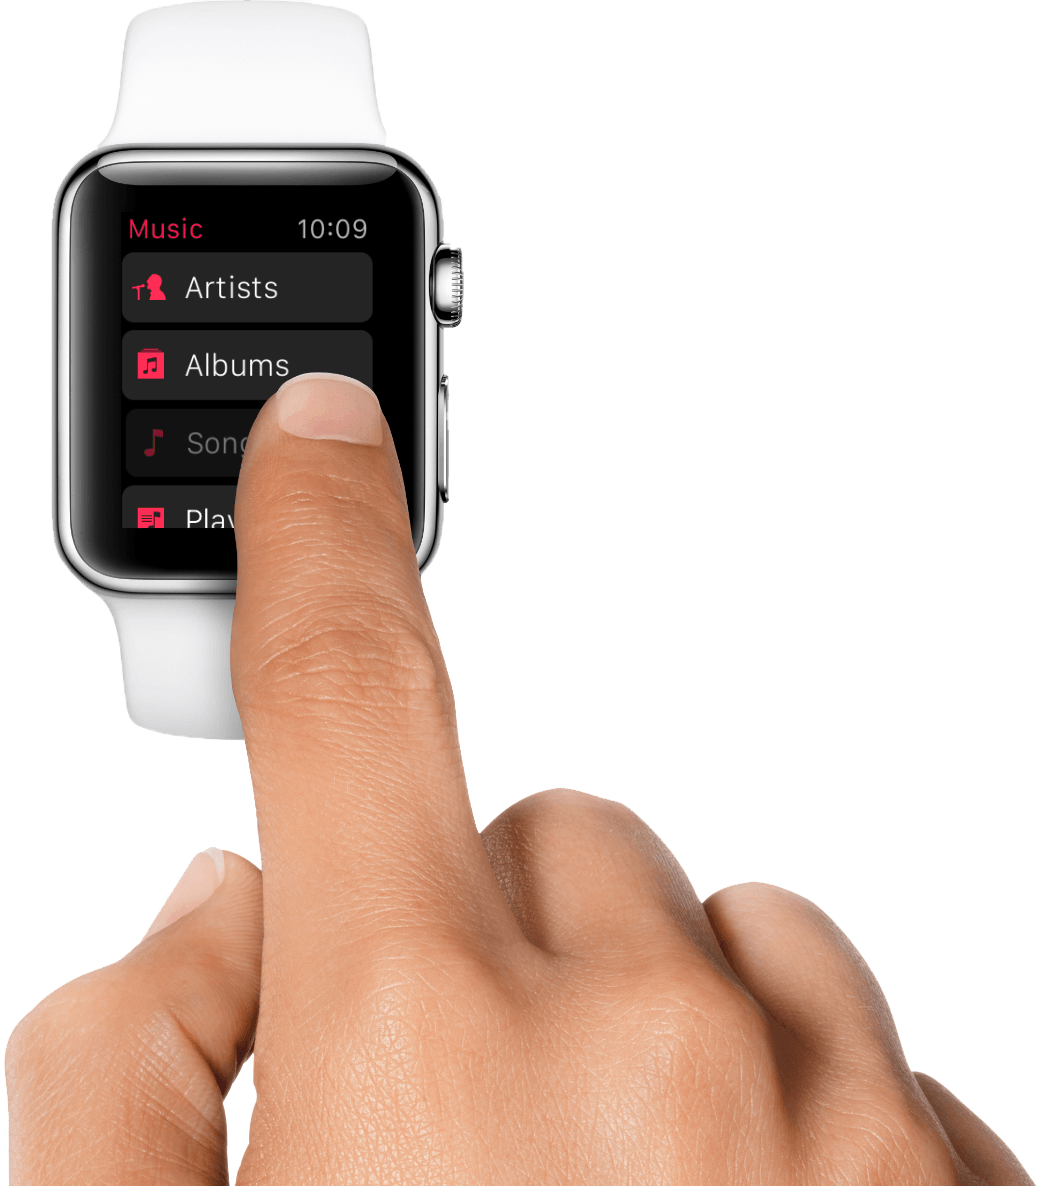
\includegraphics[width=0.2\textwidth]{figures/touch}}
    \caption{\textbf{Traditional Techniques}}
    %: 触摸屏上的单点触摸交互能够制造点按与滑动交互,而滑动交互本身又可以看做一系列连续的点按交互。此外,滑动交互仅涉及上下左右四个方向。
    \label{fig:gesture}
\end{figure}

\subsection{Tap}

Ordinary single tap on smart watches is as same as its on the smart phones.
This tap gesture as an human-computer interaction techniques has been accepted by the public for a long time, and this natural technique gains its lowest cost among the most technologies.
%屏幕的上的普通单点触控与智能手机上的方式并没有明显差异。
%这种点按方式在人机交互形式上早已被大众所接受,此种方式的用户接受成本也是最低最自然的。

However, the usability of this interaction will be reduced when the screen size reduced, in another words, we are approaching the limits when we reduce the material size and move its position on our body. According to FFitts' Law\cite{Bi:2013:FLM:2470654.2466180}:
%然而将此种交互应用在智能手表上时则极大的降低了其自身的可用性,根据触摸屏上的 FFitts' 定律\cite{Bi:2013:FLM:2470654.2466180}:

\begin{equation}
T=a+b\log_{2}{\left(\frac{A}{\sqrt{2\pi e(\sigma^2-\sigma_{a}^2)}}+1 \right)}
\end{equation}

where $\sigma$ is the standard deviation of touch position distribution, $\sigma_a$ is the absolute accuracy of the finger input, $A$ is a distance as the start point to the target center.
%其中 $\sigma$ 是触摸点分布的标准差,$\sigma_a$是输入手指的绝对精度。$A$为开始点到目标中心的距离。

Considering FFitts' Law, $A$ will be increase when screen size limited on the one hand, and $\sigma$ will not large than its on smart phone screen, on the other hand $\sigma_a$ will not change when we consider them in same object.

Thus, $T$ value will be significantly larger, which means tap interaction gains poor usability on smart watches.
%根据 FFitts' 定律我们可以看到,
%一方面,在屏幕大小及其有限的屏幕下将另一只手的手指一动到手表屏幕上会使得$A$的值很大,
%而且正由于屏幕大小的限制,$\sigma$的值不会较大甚至比手机触摸屏上的标准差还小,
%而对于同一目标而言$\sigma_a$的值又不存在变化。
%因此 $T$ 值会明显变大,即手表屏幕上的点按交互可用性并不高。

\subsection{Swipe}

Continuous tap generate swipe gesture interaction.
To process the weakness on smart watches, Apple Watch as much as possible to make the interaction to be handle be swipe gestures.
%屏幕上点按位置的连续变化形成了滑动式的交互。
%Apple Watch 在处理目标点按时的的低可用性问题时应用了滑动手势。
%例如让可交互的元素尽可能的通过滑动来进行处理。

Horizontal direction view changes can be handled by swipe gesture.
It makes interaction functions such as horizontal view change, switch back to the previous view, etc.

There is another method to take place of swipe gesture in vertical, which is using Digital Crown.
In case the vertical swipe interaction is not a subset of Digital Crown's function. It is because of Digital Crown cannot call notification center when user stay on watchOS dial interface.
%水平方向的滑动可以用于对手表界面的多个水平视图进行切换、返回上级视图等,
%垂直反向上的滑动则可以在竖直方向上滚动当前视图。
%注意,垂直方向的滑动所表达的功能并非是 Digital Crown 所具备功能的子集,
%因为在处于 watchOS 表盘界面时,上下滑动的功能会被表达为向下滑动呼出通知栏和向下滑动呼出 Glance 界面。

\section{Special Techniques}

Apple Watch introduced three more interactive hardware based on traditional interactive touch screen mode. They are Digital Crown, Force Touch and Haptic Engine, as shown in Figure \ref{fig:special}\footnote{Image Source: \url{https://developer.apple.com/watch/human-interface-guidelines/}}.

%Apple Watch 在传统触摸屏交互的基础上引入了三个全新的交互硬件,
%分别是Digital Crown、Force Touch 和 Haptic Engine,如图\ref{fig:special}所示\footnote{图片源:\url{https://developer.apple.com/watch/human-interface-guidelines/}}。

\begin{figure}[H]
    \kaishu
    \centering
    \subfigure[Digital Crown]{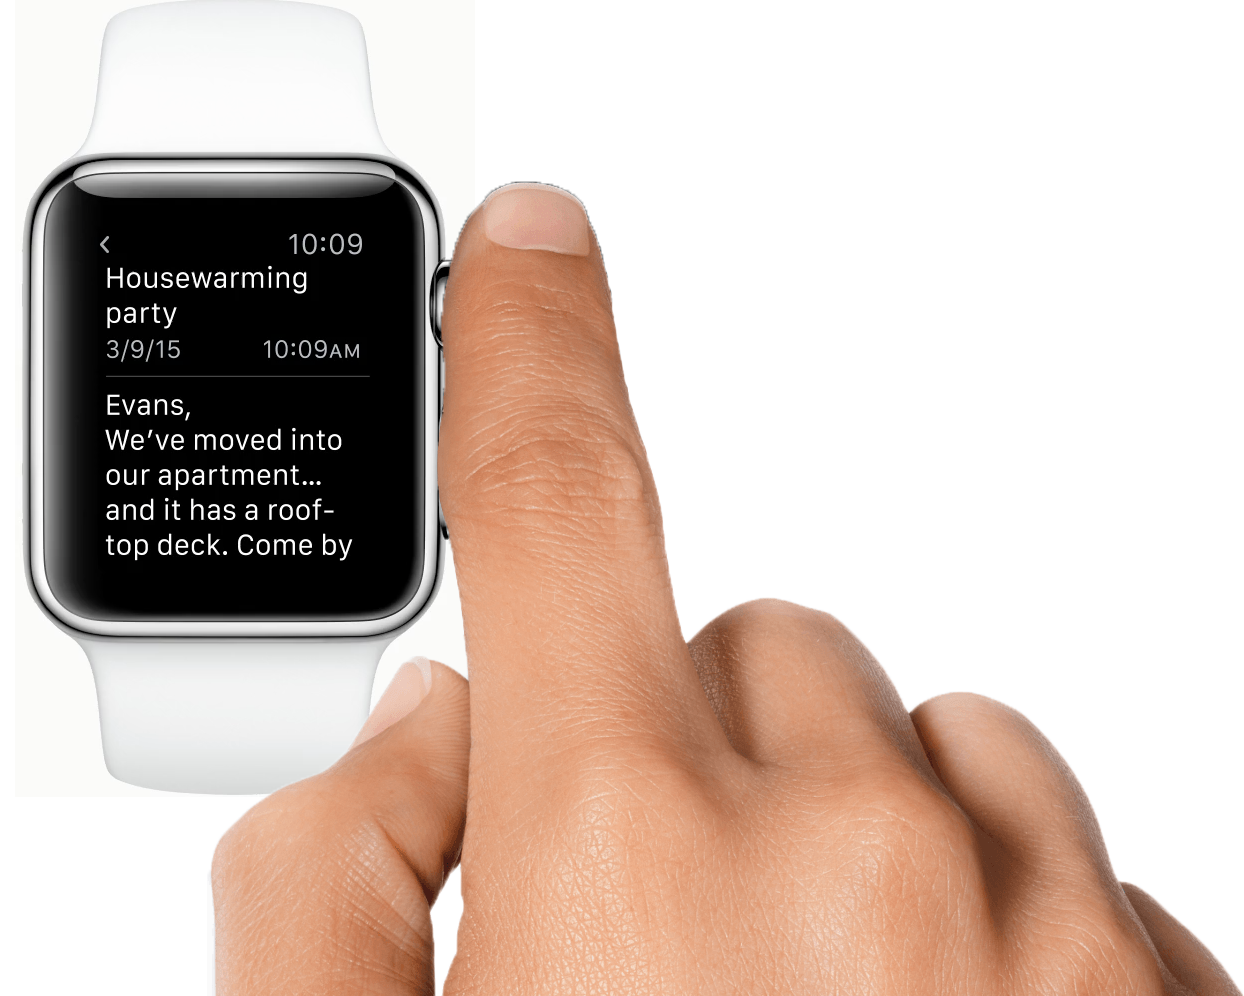
\includegraphics[width=0.3\textwidth]{figures/digital-crown}\label{fig:digital-crown}}
    \subfigure[Force Touch]{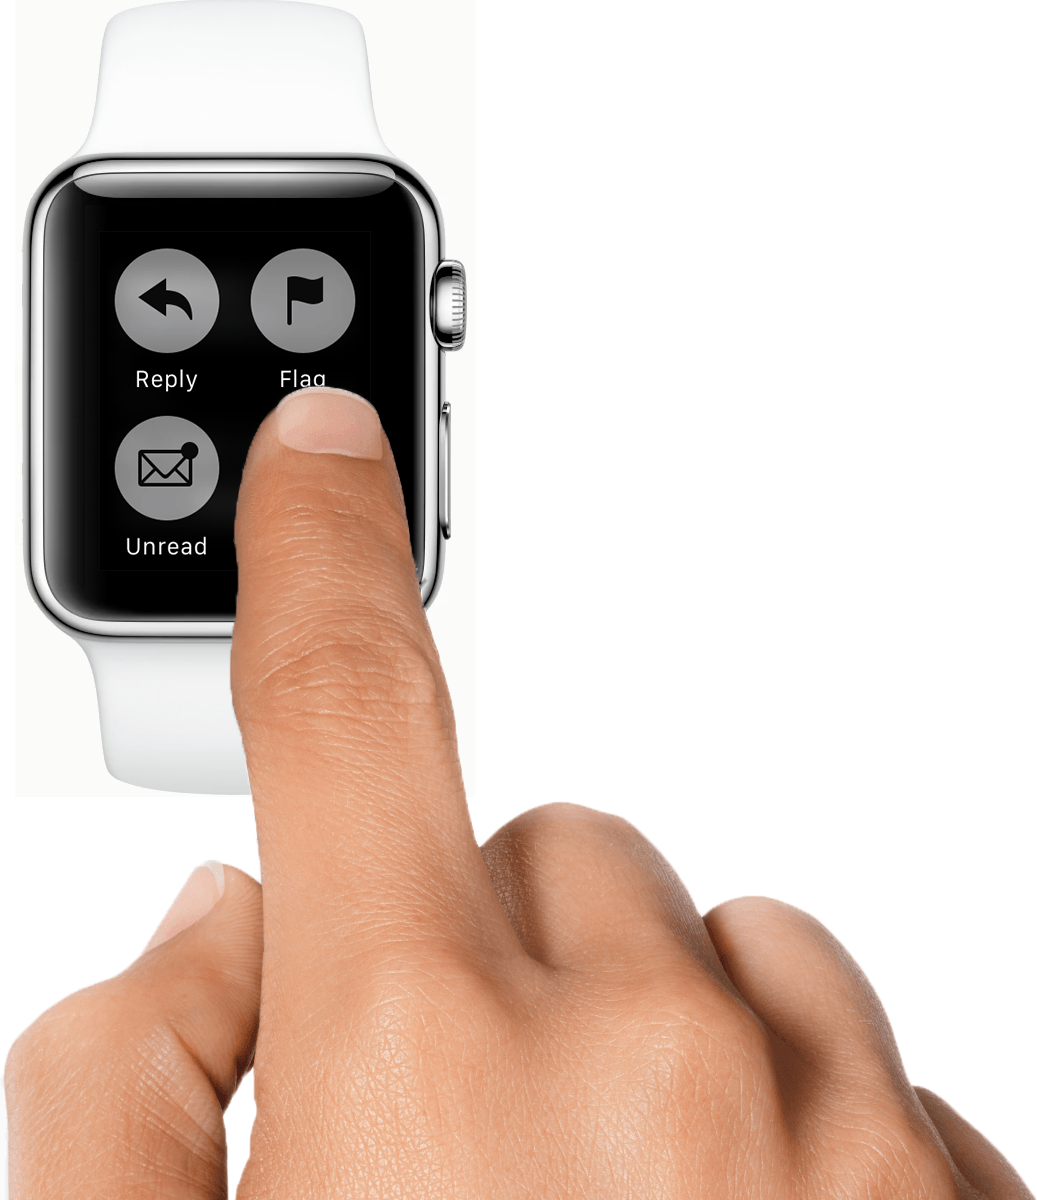
\includegraphics[width=0.2\textwidth]{figures/force-touch}\label{fig:force-touch}}
    \subfigure[Haptic Engine]{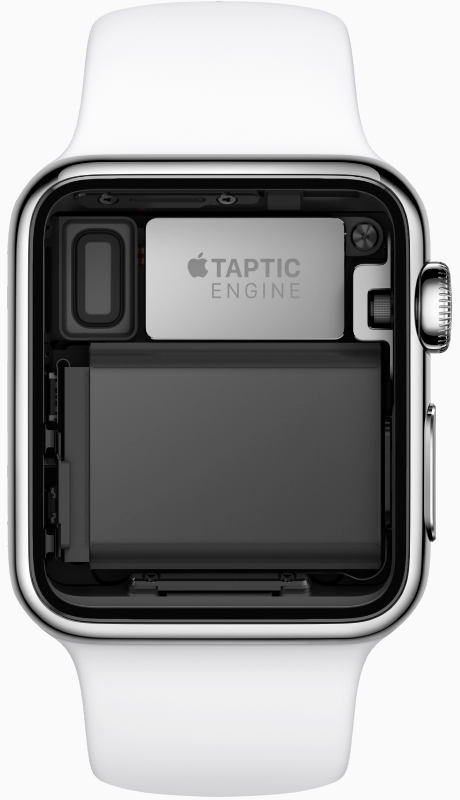
\includegraphics[width=0.15\textwidth]{figures/haptic}\label{fig:haptic}}
    \caption{\textbf{Special Techniques}: Digital Crown, Force Touch and Haptic Engine is the most significant feature in Apple Watch than other smart watch products.}
    \label{fig:special}
\end{figure}

\subsection{Digital Crown}

The Digital Crown lets users scroll content without obstructing their view of that content. It is a new interaction technique introduced by Apple Inc.
This technique is compared with the two revolutionary interaction techniques: Desktop Mouse and Multi-Touch screen when Apple Inc. were introducing this, which means Apple Inc. maintain Digital Crown is a revolutionary technique on smart watches.
%Digital Crown 是苹果公司在Apple Watch上推出的一个全新的交互技术,
%苹果公司在推出此项交互的技术时,将其对比了在人机交互历史中的两个革命性的交互技术:
%鼠标和触摸屏,这意味着苹果公司认为,Digital Crown 是一项在手表上的革命性交互方式。

This interaction take the advantage of traditional watch clock function, which is visible but also insufficiency.
In a conventional watch, the clock dial in the normal state does not have any function, only when the knob is pulled out and the only function is adjusting time. This device is uselessness in the most of time. It's a typical demand-driven design. Designers are not carefully think about its existence but just habitual in use.
%这种交互方式利用了传统手表的时钟旋钮在功能可见性上的不足。
%在传统手表中,时钟旋钮在普通状态下不具备任何功能,只有当旋钮被从里向外拉出时,才具备调节时间的功能。
%这一装置在大部分时间里都不能发挥自身的作用,是一个典型的需求驱动型设计,
%并没有仔细考虑过其自身的存在方式,只是习惯性沿用。

On the Apple Watch, content are displayed vertically and it's restricted on a fixed width.
When Digital Crown scroll up and down, the content will be change in vertical direction, as shown in Figure \ref{fig:digital-crown}; Besides, Digital Crown can also adjust the playback volume of the music.
%而在 Apple Watch 上,信息呈现的方式以流式进行纵向展示,
%所有呈现的内容被限制在一个宽度固定、纵向可伸缩的屏幕区域里。
%这时,Digital Crown 便能发挥其旋钮的功能。
%当产生旋转时,内容在竖直方向上进行移动,从而呈现更多的内容,如图\ref{fig:digital-crown};
%并且,在交互情景发生变化时,Digital Crown 能够表达出不同的交互指令,
%例如在音乐播放界面时,Digital Crown 的旋转能够调节播放音乐的音量。

\subsection{Force Touch}

Apple Watch display not only senses a touch, it senses the force applied by user's finger and responds accordingly. Force Touch is the first applying in consumer products. In academia, this technology has been studied years.

\cite{Boring:2012ea,Buschek:2015cd,Vogel:2007:STO:1240624.1240727} studied how to enhance touch feedback, force level and touch area. Force Touch applied them into Apple Watch.
%Force Touch 这项交互技术是首次在民用消费品中出现。在学术界中,对触摸的感知被研究了多年,
%\cite{Boring:2012ea,Buschek:2015cd,Vogel:2007:STO:1240624.1240727}等文献研究了触觉感知如何在触摸屏上进行增强,
%包括感觉反馈、触摸面积的测量、触摸力度和精度等等,而 Force Touch 就是触摸力度的实际体现。

Force Touch contains two level of touch behavior, the first level is traditional touch action, it can reconize normal tap gesture;
The second level is actually Force Touch, at this moment, user need increase finger's force value, then watchOS will response and handle this interaction.
As illustrate on Figure \ref{fig:force-touch}, obviously, this interaction is a typical interaction mode without affordance, these functions are perceptible only the operation performed.
%Force Touch 一共将触摸行为分为了两个等级,第一触摸等级就是传统意义上的触摸行为,手指轻触屏幕时即可被感知;
%第二触摸等级就是 Force Touch,这时需要用户将触摸屏幕的力度提升到一个级别后,系统才会进行响应进一步处理交互,
%如图\ref{fig:force-touch}。然而,这是一个典型的不具备功能可见性的交互形式,只有当操作被执行后,才能进行后续的交互。

\subsection{Haptic Engine}

Haptic Engine is built-in vibration member, as illustrate in Figure \ref{fig:haptic}.
It is an important way to get the user's attention and to convey important information.
%Haptic Engine 是一个内置的震动部件,如图\ref{fig:haptic}。通过这个部件对手腕传达的震动信息,
Haptic Engine are not just a normal vibration but also a high precision hardware, it can transfer user's heartbeat to another, make user feel Force Touch perform notification, then enhance the user experiences of Apple Watch.
%可以进一步扩大用户与手表进行交互时的反馈。
%例如,当用户成功实施 Force Touch 后 Haptic Engine 能够给予用户不同层级的反馈,
%让用户亲自感受到 Force Touch 的实施成功;
%Haptic Engine 能够在不同用户之间分享彼此的心跳频率时自行调节振动的幅度和速度,达到真实的模拟心跳,进而显著提升 Apple Watch 的用户体验。
Thus, whatever how to modify current interaction mode into alternative design, we should always provide the Haptic Feedback to users.
%当我们对现有交互进行备择设计时,无论交互方式如何更改,都应该向用户提供震动反馈来提醒用户操作是否成功。
In other words, Haptic Engine vibration feedback is provided to be the key of alternative interaction design.
%换句话说,Haptic Engine 所提供的震动反馈是进行非接触式备择设计的关键所在。

\section{Other Techniques}

In addition, except the basic interaction techniques above, there are two highest priority interactive method on Apple Watch, as Figure \ref{fig:others} illustrated\footnote{图片源:\url{https://developer.apple.com/watch/human-interface-guidelines/}}.
%除了以上的基础交互手段外,在 Apple Watch 上还有两个最高优先级的交互方式,如图\ref{fig:others}所示\footnote{图片源:\url{https://developer.apple.com/watch/human-interface-guidelines/}}。

\begin{figure}[H]
    \kaishu
    \centering
    \subfigure[Side Button]{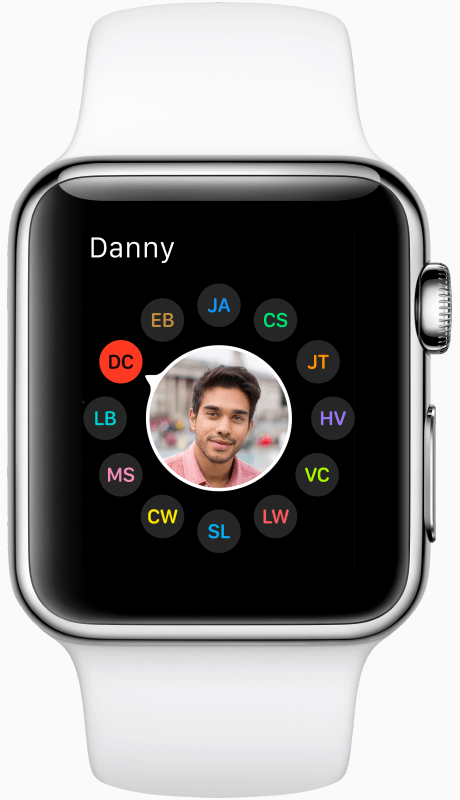
\includegraphics[width=0.2\textwidth]{figures/side}\label{fig:side}}
    \subfigure[Voice Control]{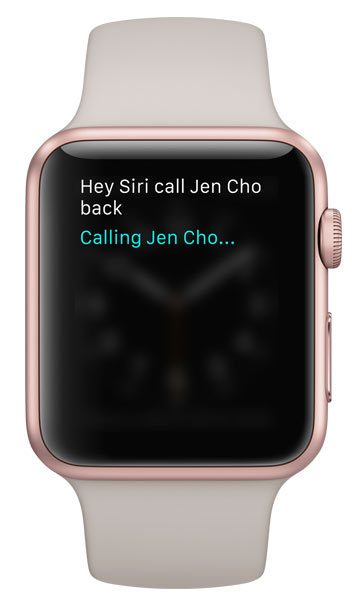
\includegraphics[width=0.2\textwidth]{figures/siri}\label{fig:siri}}
    \caption{\textbf{Other interaction techniques}:Side button gives us the top-level interaction for Friends,and Siri is the only text entry on the Apple Watch.}
    \label{fig:others}
\end{figure}

Two buttons on the side of Apple Watch actually is the highest priority of interactions, because wherever the user in watchOS, it alway takes user to the Friend view and Siri interface (Note that a single tap of Digital Crown is not able to mark as highest priority interaction, because a single tap perform results may not be unique: It may be in the dial, or it may be in total App Interfaces).
%Apple Watch 侧面的两个按钮实际上是 Apple Watch 里所有交互中优先级最高的交互方式,这是因为无论用户在 watchOS 中所处的位置在哪儿,都能够通过这两个方法执行固定的交互指令(注意,单次点按 Digital Crown 并不能够作为最高优先级的交互,因为单次点按 Digital Crown 后用户所处的位置可能不唯一:可能会处于表盘,也可能处于 App 总界面)。

\subsection{Side Button}

Apple Inc. may have noticed that the Apple Watch application gains its complexity and inconvenience, they follows the design of the power button on smart phone and they still add another physical buttons called Side Button next to the Digital Crown, as Figure \ref{fig:side}.
%苹果公司可能注意到了在 Apple Watch 上对应用操作的延时复杂性和不便,沿用了手机上电源键的设计,
%在已经存在 Digital Crown 按键的基础上依然添加了另一个实体按键,如图\ref{fig:side}。

The existence of two different pieces of renovation interactive content inside the Side Button, when user perform a button click, it will access the Friends screen. From this screen, they can call friends, send message, or interact by sending sketches, taps, and even their heartbeat. When user press the Side Button twice, it will access the Apple Pay.
%该颗改建存在两个不同的交互内容,当按下该按键一次时,按键会呼出常用联系人列表,
%方便通过 Apple Watch 拨打电话及发送讯息等;
%当连续按下改建两次时,如果当前 Apple Watch 绑定 Apple Pay 银行卡时,
%能够呼出默认银行卡进行 Apple Pay 支付。

\subsection{Voice Control}

Although there are a lot of input method design on wearable devices,
but Apple Watch did not take any of them on watchOS, text input entrance
(even virtual keyboard) are not directly setup into watchOS, thus Siri becomes
the only interface allows user input text by speaking, as shown in Figure \ref{fig:siri}.
%尽管对于穿戴式设备的输入方式有很多设计,但是在 watchOS 上是没有直接的(哪怕是屏幕上的键盘)文本输入入口。
%因此,Siri 成了唯一一个能够向 watchOS 输入文本的接口,如图\ref{fig:siri}。

For weak up Siri, user have two way to do. One is say "Hey Siri" when Apple Watch is
on awake state; Another is give a long-press to Digital Crown.
%watchOS 上的 Siri 有两种呼出方式,一种是在 Apple Watch 处于唤醒状态下时说出『Hey Siri』;
%另一种则是长按 Digital Crown。

However, no matter which way to choose, text input results will not ideal.
This is because Siri's nature language recognition process based on statistics and
it always require a paired iPhone to access Internet.
Any part of this gets a problem can crash the whole input progress.
%然而,无论是其中的哪种方式,最后的文字输入效果都不理想。
%这是因为 Siri 依赖自然语言的识别处理,同时还需要一个配对的手机进行网络访问。
%这其中只要任何一个环节出问题便不能完成文字的输入。

It is worth mentioning that the interaction method we discussed above,
only Siri voice control is a contact-free  interaction design.
%值得一提的是,在上文提到的所有的交互方式中,只有语音控制是非接触式的交互设计。

\cleardoublepage
